\subsection{Functions}

\begin{enumerate}
	\item 
	\begin{enumerate}[topsep=0ex,itemsep=0ex,partopsep=1ex,parsep=1ex]
		\item[(a)] A function is defined by the equation $f(x) = mx^2 + nx + k$. If $f(2) = 7$, $f(0) = -3$, and $f(-1) = 2$, 
		\begin{enumerate}[topsep=0ex,itemsep=0ex,partopsep=1ex,parsep=1ex]
			\item[i)] Determine the values of $m$, $n$, and $k$. 
			\item[ii)] Find the domain and range of $f(x)$
		\end{enumerate}
		
		\item[(b)] 
		\begin{enumerate}[topsep=0ex,itemsep=0ex,partopsep=1ex,parsep=1ex]
			\item[i)] Sketch the graph of the rational function $g(x) = \frac{1}{4x - 8}$
			\item[ii)] What are the values of $x$ and $y$ for which $g(x)$ is defined?
		\end{enumerate}
	\end{enumerate}

	\item
	\begin{enumerate}[topsep=0ex,itemsep=0ex,partopsep=1ex,parsep=1ex]
		\item[(a)] Given that $f(x) = 3x - 1$ and $g(x) = \sqrt{2x - 1}$. Find, 
		\begin{enumerate}[topsep=0ex,itemsep=0ex,partopsep=1ex,parsep=1ex]
			\item[i)] $f \circ g(25)$ 
			\item[ii)] $g \circ f(14)$
		\end{enumerate}
		
		\item[(b)] 
		\begin{enumerate}[topsep=0ex,itemsep=0ex,partopsep=1ex,parsep=1ex]
			\item[i)] Verify that $x + 4$ is not a factor of the polynomial function $f(x) = 2x^3 - 15x^2 + 24$
			\item[ii)] Describe the nature of the stationary points of the function $f(x) = 2x^3 - 15x^2 + 24x$, hence show them one the graph
		\end{enumerate}
	\end{enumerate}
	
	\item
	\begin{enumerate}[topsep=0ex,itemsep=0ex,partopsep=1ex,parsep=1ex]
		\item[(a)] Find the coordinates of the points where the line $y - 2x +5 = 0$ meets the curve $3x^2 - 4y^2 = 10 + xy$.
		
		\item[(b)] The graph of the function $f(x)$ is given below, \\
		\begin{center}
			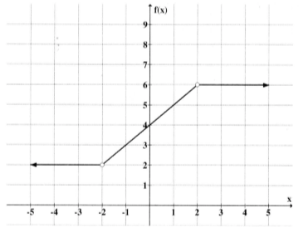
\includegraphics[width=0.5\textwidth]{./img/math_BAM_functions_1.png}
		\end{center}
		Use the graph to determine:
		\begin{enumerate}[topsep=0ex,itemsep=0ex,partopsep=1ex,parsep=1ex]
			\item[i)] The function $f(x)$
			\item[ii)] The domain and range of $f(x)$
		\end{enumerate}
		
		\item[(c)] Find the asymptotes and the intercepts of the function $f(x) = \frac{3x - 7}{x + 2}$ and then sketch its graph. 
	\end{enumerate}

\end{enumerate}











